\documentclass{standalone}
\usepackage{tikz}
\usetikzlibrary{patterns, positioning}
\usepackage[sfdefault]{ClearSans} %% option 'sfdefault' activates Clear Sans as the default text font
\usepackage[T1]{fontenc}

\begin{document}
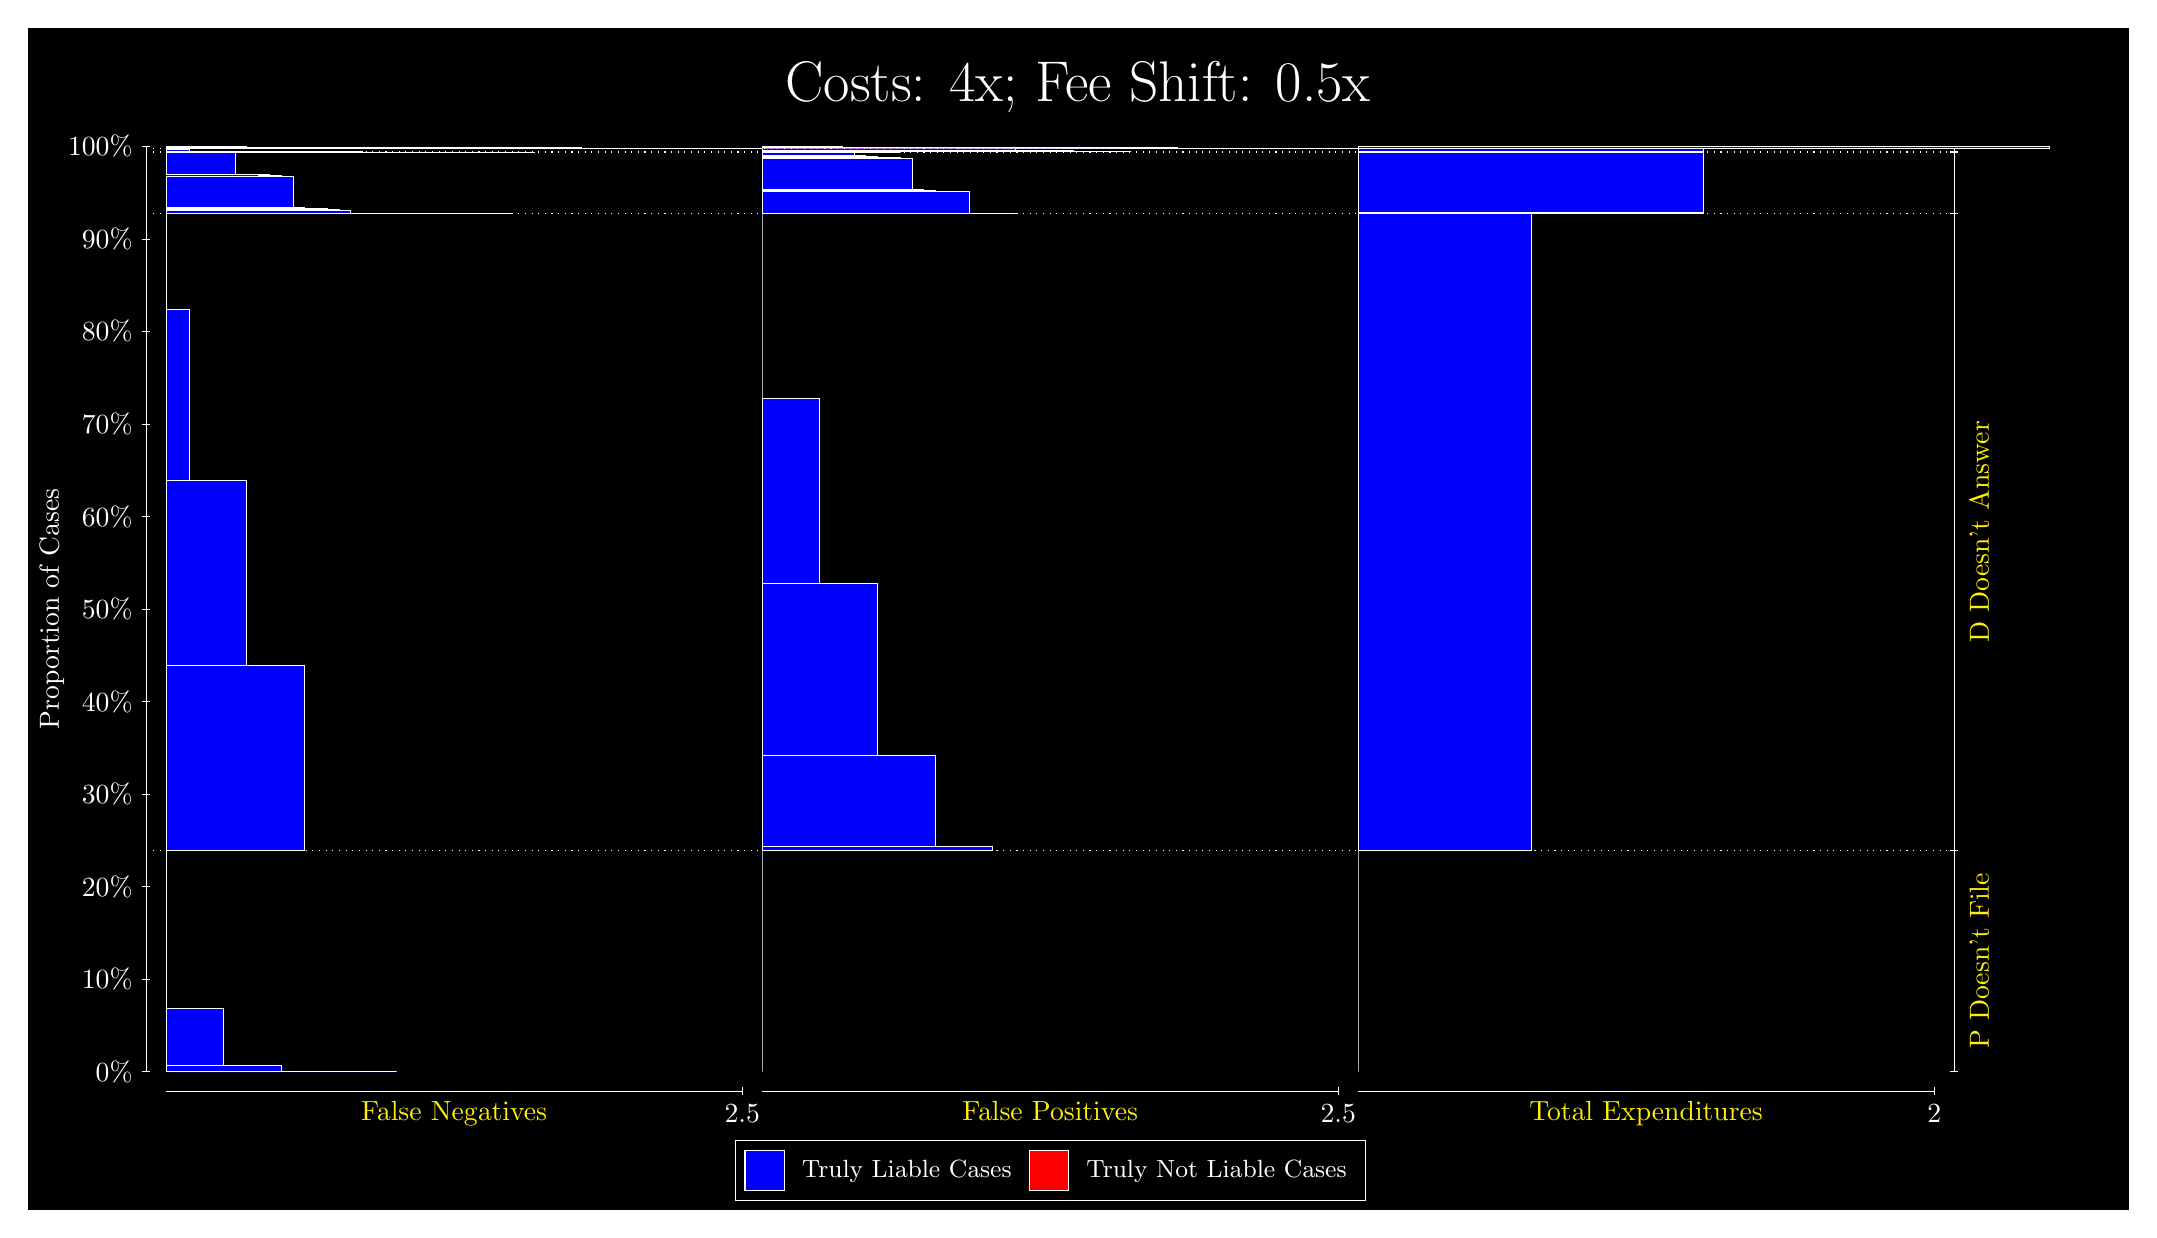
\begin{tikzpicture}
\draw[fill=black] (0,0) rectangle (26.667,15);
\draw[text=white] (0,13.5) rectangle (26.667,15) node[midway] {\huge Costs: 4x; Fee Shift: 0.5x};
\draw[white, very thin] (1.5,1.75) -- (1.5,13.5);
\node[rotate=90, text=white, anchor=center] at (0.3, 7.625) {Proportion of Cases};
\draw[white, very thin] (1.45,1.75) -- (1.55,1.75);
\node[text=white, anchor=east] at (1.45, 1.75) {0\%};
\draw[white, very thin] (1.45,2.925) -- (1.55,2.925);
\node[text=white, anchor=east] at (1.45, 2.925) {10\%};
\draw[white, very thin] (1.45,4.1) -- (1.55,4.1);
\node[text=white, anchor=east] at (1.45, 4.1) {20\%};
\draw[white, very thin] (1.45,5.275) -- (1.55,5.275);
\node[text=white, anchor=east] at (1.45, 5.275) {30\%};
\draw[white, very thin] (1.45,6.45) -- (1.55,6.45);
\node[text=white, anchor=east] at (1.45, 6.45) {40\%};
\draw[white, very thin] (1.45,7.625) -- (1.55,7.625);
\node[text=white, anchor=east] at (1.45, 7.625) {50\%};
\draw[white, very thin] (1.45,8.8) -- (1.55,8.8);
\node[text=white, anchor=east] at (1.45, 8.8) {60\%};
\draw[white, very thin] (1.45,9.975) -- (1.55,9.975);
\node[text=white, anchor=east] at (1.45, 9.975) {70\%};
\draw[white, very thin] (1.45,11.15) -- (1.55,11.15);
\node[text=white, anchor=east] at (1.45, 11.15) {80\%};
\draw[white, very thin] (1.45,12.325) -- (1.55,12.325);
\node[text=white, anchor=east] at (1.45, 12.325) {90\%};
\draw[white, very thin] (1.45,13.5) -- (1.55,13.5);
\node[text=white, anchor=east] at (1.45, 13.5) {100\%};

\draw[white, very thin] (24.457,1.75) -- (24.457,13.5);
\draw[white, very thin] (24.407,1.75) -- (24.507,1.75);
\node[anchor=west] at (24.407, 1.75) {};
\draw[white, very thin] (24.407,4.5558) -- (24.507,4.5558);
\node[anchor=west] at (24.407, 4.5558) {};
\draw[white, very thin] (24.407,12.651) -- (24.507,12.651);
\node[anchor=west] at (24.407, 12.651) {};
\draw[white, very thin] (24.407,13.423) -- (24.507,13.423);
\node[anchor=west] at (24.407, 13.423) {};
\draw[white, very thin] (24.407,13.439) -- (24.507,13.439);
\node[anchor=west] at (24.407, 13.439) {};
\draw[white, very thin] (24.407,13.473) -- (24.507,13.473);
\node[anchor=west] at (24.407, 13.473) {};
\draw[white, very thin] (24.407,13.5) -- (24.507,13.5);
\node[anchor=west] at (24.407, 13.5) {};

\draw[white, very thin, fill=blue] (1.75,1.75) rectangle (4.6775,1.75);
\draw[white, very thin, fill=blue] (1.75,1.75) rectangle (3.9457,1.7507);
\draw[white, very thin, fill=blue] (1.75,1.7507) rectangle (3.2138,1.8342);
\draw[white, very thin, fill=blue] (1.75,1.8342) rectangle (2.4819,2.5535);
\draw[white, very thin, fill=red] (1.75,2.5535) rectangle (1.75,2.5535);
\draw[white, very thin, fill=blue] (1.75,2.5535) rectangle (1.75,4.5558);
\draw[white, very thin, fill=blue] (1.75,4.5558) rectangle (3.5065,6.9058);
\draw[white, very thin, fill=blue] (1.75,6.9058) rectangle (2.7746,9.2543);
\draw[white, very thin, fill=blue] (1.75,9.2543) rectangle (2.0428,11.436);
\draw[white, very thin, fill=red] (1.75,11.436) rectangle (1.75,11.436);
\draw[white, very thin, fill=blue] (1.75,11.436) rectangle (1.75,12.651);
\draw[white, very thin, fill=blue] (1.75,12.651) rectangle (6.1413,12.651);
\draw[white, very thin, fill=blue] (1.75,12.651) rectangle (5.8486,12.651);
\draw[white, very thin, fill=blue] (1.75,12.651) rectangle (5.5558,12.651);
\draw[white, very thin, fill=blue] (1.75,12.651) rectangle (5.4094,12.651);
\draw[white, very thin, fill=blue] (1.75,12.651) rectangle (5.2631,12.651);
\draw[white, very thin, fill=blue] (1.75,12.651) rectangle (5.1167,12.651);
\draw[white, very thin, fill=blue] (1.75,12.651) rectangle (4.9703,12.651);
\draw[white, very thin, fill=blue] (1.75,12.651) rectangle (4.8239,12.651);
\draw[white, very thin, fill=blue] (1.75,12.651) rectangle (4.6775,12.651);
\draw[white, very thin, fill=blue] (1.75,12.651) rectangle (4.5312,12.651);
\draw[white, very thin, fill=blue] (1.75,12.651) rectangle (4.3848,12.652);
\draw[white, very thin, fill=blue] (1.75,12.652) rectangle (4.2384,12.652);
\draw[white, very thin, fill=blue] (1.75,12.652) rectangle (4.092,12.689);
\draw[white, very thin, fill=blue] (1.75,12.689) rectangle (3.9457,12.698);
\draw[white, very thin, fill=blue] (1.75,12.698) rectangle (3.7993,12.711);
\draw[white, very thin, fill=blue] (1.75,12.711) rectangle (3.6529,12.717);
\draw[white, very thin, fill=blue] (1.75,12.717) rectangle (3.5065,12.724);
\draw[white, very thin, fill=blue] (1.75,12.724) rectangle (3.3602,13.114);
\draw[white, very thin, fill=blue] (1.75,13.114) rectangle (3.2138,13.126);
\draw[white, very thin, fill=blue] (1.75,13.126) rectangle (3.0674,13.139);
\draw[white, very thin, fill=blue] (1.75,13.139) rectangle (2.921,13.14);
\draw[white, very thin, fill=blue] (1.75,13.14) rectangle (2.7746,13.143);
\draw[white, very thin, fill=blue] (1.75,13.143) rectangle (2.6283,13.423);
\draw[white, very thin, fill=blue] (1.75,13.423) rectangle (2.3355,13.423);
\draw[white, very thin, fill=blue] (1.75,13.423) rectangle (2.0428,13.423);
\draw[white, very thin, fill=red] (1.75,13.423) rectangle (1.75,13.423);
\draw[white, very thin, fill=blue] (1.75,13.423) rectangle (6.4341,13.423);
\draw[white, very thin, fill=blue] (1.75,13.423) rectangle (5.7022,13.423);
\draw[white, very thin, fill=blue] (1.75,13.423) rectangle (4.9703,13.425);
\draw[white, very thin, fill=blue] (1.75,13.425) rectangle (4.2384,13.438);
\draw[white, very thin, fill=blue] (1.75,13.438) rectangle (3.5065,13.439);
\draw[white, very thin, fill=red] (1.75,13.439) rectangle (1.75,13.439);
\draw[white, very thin, fill=blue] (1.75,13.439) rectangle (3.5065,13.439);
\draw[white, very thin, fill=blue] (1.75,13.439) rectangle (2.7746,13.439);
\draw[white, very thin, fill=blue] (1.75,13.439) rectangle (2.0428,13.46);
\draw[white, very thin, fill=red] (1.75,13.46) rectangle (1.75,13.46);
\draw[white, very thin, fill=blue] (1.75,13.46) rectangle (1.75,13.473);
\draw[white, very thin, fill=blue] (1.75,13.473) rectangle (9.9471,13.473);
\draw[white, very thin, fill=blue] (1.75,13.473) rectangle (9.2152,13.473);
\draw[white, very thin, fill=blue] (1.75,13.473) rectangle (8.4834,13.473);
\draw[white, very thin, fill=blue] (1.75,13.473) rectangle (7.7515,13.479);
\draw[white, very thin, fill=blue] (1.75,13.479) rectangle (7.0196,13.488);
\draw[white, very thin, fill=blue] (1.75,13.488) rectangle (6.2877,13.489);
\draw[white, very thin, fill=blue] (1.75,13.489) rectangle (5.7022,13.489);
\draw[white, very thin, fill=blue] (1.75,13.489) rectangle (4.9703,13.489);
\draw[white, very thin, fill=blue] (1.75,13.489) rectangle (4.2384,13.489);
\draw[white, very thin, fill=blue] (1.75,13.489) rectangle (3.5065,13.493);
\draw[white, very thin, fill=blue] (1.75,13.493) rectangle (2.7746,13.499);
\draw[white, very thin, fill=blue] (1.75,13.499) rectangle (2.0428,13.5);
\draw[white, very thin, fill=red] (1.75,13.5) rectangle (1.75,13.5);
\draw[white, very thin, fill=blue] (1.75,13.5) rectangle (1.75,13.5);
\draw[white, very thin, fill=red] (9.3189,1.75) rectangle (9.3189,1.75);
\draw[white, very thin, fill=blue] (9.3189,1.75) rectangle (9.3189,4.5558);
\draw[white, very thin, fill=red] (9.3189,4.5558) rectangle (12.246,4.5558);
\draw[white, very thin, fill=blue] (9.3189,4.5558) rectangle (12.246,4.6098);
\draw[white, very thin, fill=blue] (9.3189,4.6098) rectangle (11.515,5.7711);
\draw[white, very thin, fill=blue] (9.3189,5.7711) rectangle (10.783,7.9528);
\draw[white, very thin, fill=blue] (9.3189,7.9528) rectangle (10.051,10.301);
\draw[white, very thin, fill=blue] (9.3189,10.301) rectangle (9.3189,12.651);
\draw[white, very thin, fill=red] (9.3189,12.651) rectangle (12.539,12.651);
\draw[white, very thin, fill=blue] (9.3189,12.651) rectangle (12.539,12.651);
\draw[white, very thin, fill=red] (9.3189,12.651) rectangle (12.246,12.651);
\draw[white, very thin, fill=blue] (9.3189,12.651) rectangle (12.246,12.651);
\draw[white, very thin, fill=red] (9.3189,12.651) rectangle (11.954,12.651);
\draw[white, very thin, fill=blue] (9.3189,12.651) rectangle (11.954,12.931);
\draw[white, very thin, fill=blue] (9.3189,12.931) rectangle (11.807,12.934);
\draw[white, very thin, fill=red] (9.3189,12.934) rectangle (11.661,12.934);
\draw[white, very thin, fill=blue] (9.3189,12.934) rectangle (11.661,12.935);
\draw[white, very thin, fill=blue] (9.3189,12.935) rectangle (11.515,12.948);
\draw[white, very thin, fill=red] (9.3189,12.948) rectangle (11.368,12.948);
\draw[white, very thin, fill=blue] (9.3189,12.948) rectangle (11.368,12.96);
\draw[white, very thin, fill=blue] (9.3189,12.96) rectangle (11.222,13.35);
\draw[white, very thin, fill=blue] (9.3189,13.35) rectangle (11.075,13.357);
\draw[white, very thin, fill=blue] (9.3189,13.357) rectangle (10.929,13.363);
\draw[white, very thin, fill=blue] (9.3189,13.363) rectangle (10.783,13.376);
\draw[white, very thin, fill=blue] (9.3189,13.376) rectangle (10.636,13.385);
\draw[white, very thin, fill=blue] (9.3189,13.385) rectangle (10.49,13.422);
\draw[white, very thin, fill=blue] (9.3189,13.422) rectangle (10.344,13.422);
\draw[white, very thin, fill=blue] (9.3189,13.422) rectangle (10.197,13.423);
\draw[white, very thin, fill=blue] (9.3189,13.423) rectangle (10.051,13.423);
\draw[white, very thin, fill=blue] (9.3189,13.423) rectangle (9.9044,13.423);
\draw[white, very thin, fill=blue] (9.3189,13.423) rectangle (9.758,13.423);
\draw[white, very thin, fill=blue] (9.3189,13.423) rectangle (9.6116,13.423);
\draw[white, very thin, fill=blue] (9.3189,13.423) rectangle (9.4652,13.423);
\draw[white, very thin, fill=blue] (9.3189,13.423) rectangle (9.3189,13.423);
\draw[white, very thin, fill=red] (9.3189,13.423) rectangle (11.075,13.423);
\draw[white, very thin, fill=blue] (9.3189,13.423) rectangle (11.075,13.423);
\draw[white, very thin, fill=blue] (9.3189,13.423) rectangle (10.344,13.436);
\draw[white, very thin, fill=blue] (9.3189,13.436) rectangle (9.6116,13.439);
\draw[white, very thin, fill=blue] (9.3189,13.439) rectangle (9.3189,13.439);
\draw[white, very thin, fill=red] (9.3189,13.439) rectangle (14.003,13.439);
\draw[white, very thin, fill=blue] (9.3189,13.439) rectangle (14.003,13.439);
\draw[white, very thin, fill=blue] (9.3189,13.439) rectangle (13.271,13.452);
\draw[white, very thin, fill=blue] (9.3189,13.452) rectangle (12.539,13.472);
\draw[white, very thin, fill=blue] (9.3189,13.472) rectangle (11.807,13.473);
\draw[white, very thin, fill=blue] (9.3189,13.473) rectangle (11.075,13.473);
\draw[white, very thin, fill=red] (9.3189,13.473) rectangle (17.516,13.473);
\draw[white, very thin, fill=blue] (9.3189,13.473) rectangle (17.516,13.473);
\draw[white, very thin, fill=red] (9.3189,13.473) rectangle (16.784,13.473);
\draw[white, very thin, fill=blue] (9.3189,13.473) rectangle (16.784,13.473);
\draw[white, very thin, fill=red] (9.3189,13.473) rectangle (16.052,13.473);
\draw[white, very thin, fill=blue] (9.3189,13.473) rectangle (16.052,13.473);
\draw[white, very thin, fill=red] (9.3189,13.473) rectangle (15.32,13.473);
\draw[white, very thin, fill=blue] (9.3189,13.473) rectangle (15.32,13.479);
\draw[white, very thin, fill=blue] (9.3189,13.479) rectangle (14.588,13.484);
\draw[white, very thin, fill=blue] (9.3189,13.484) rectangle (13.857,13.484);
\draw[white, very thin, fill=blue] (9.3189,13.484) rectangle (13.125,13.484);
\draw[white, very thin, fill=blue] (9.3189,13.484) rectangle (12.393,13.484);
\draw[white, very thin, fill=red] (9.3189,13.484) rectangle (11.807,13.484);
\draw[white, very thin, fill=blue] (9.3189,13.484) rectangle (11.807,13.484);
\draw[white, very thin, fill=red] (9.3189,13.484) rectangle (11.075,13.484);
\draw[white, very thin, fill=blue] (9.3189,13.484) rectangle (11.075,13.494);
\draw[white, very thin, fill=blue] (9.3189,13.494) rectangle (10.344,13.5);
\draw[white, very thin, fill=blue] (9.3189,13.5) rectangle (9.6116,13.5);
\draw[white, very thin, fill=blue] (9.3189,13.5) rectangle (9.3189,13.5);
\draw[white, very thin, fill=red] (16.888,1.75) rectangle (16.888,1.75);
\draw[white, very thin, fill=blue] (16.888,1.75) rectangle (16.888,4.5558);
\draw[white, very thin, fill=red] (16.888,4.5558) rectangle (19.083,4.5558);
\draw[white, very thin, fill=blue] (16.888,4.5558) rectangle (19.083,12.651);
\draw[white, very thin, fill=red] (16.888,12.651) rectangle (21.279,12.651);
\draw[white, very thin, fill=blue] (16.888,12.651) rectangle (21.279,12.662);
\draw[white, very thin, fill=red] (16.888,12.662) rectangle (21.279,12.662);
\draw[white, very thin, fill=blue] (16.888,12.662) rectangle (21.279,13.423);
\draw[white, very thin, fill=red] (16.888,13.423) rectangle (21.279,13.423);
\draw[white, very thin, fill=blue] (16.888,13.423) rectangle (21.279,13.439);
\draw[white, very thin, fill=red] (16.888,13.439) rectangle (21.279,13.439);
\draw[white, very thin, fill=blue] (16.888,13.439) rectangle (21.279,13.473);
\draw[white, very thin, fill=red] (16.888,13.473) rectangle (25.67,13.473);
\draw[white, very thin, fill=blue] (16.888,13.473) rectangle (25.67,13.5);
\draw[white, dotted] (1.5,4.5558) -- (24.457,4.5558);
\draw[white, dotted] (1.5,12.651) -- (24.457,12.651);
\draw[white, dotted] (1.5,13.423) -- (24.457,13.423);
\draw[white, dotted] (1.5,13.439) -- (24.457,13.439);
\draw[white, dotted] (1.5,13.473) -- (24.457,13.473);
\draw[white, very thin] (1.75,1.5) -- (9.0689,1.5);
\node[text=yellow, anchor=north] at (5.4094, 1.5) {False Negatives};
\draw[white, very thin] (9.0689,1.45) -- (9.0689,1.55);
\node[text=white, anchor=north] at (9.0689, 1.45) {2.5};

\draw[white, very thin] (9.3189,1.5) -- (16.638,1.5);
\node[text=yellow, anchor=north] at (12.978, 1.5) {False Positives};
\draw[white, very thin] (16.638,1.45) -- (16.638,1.55);
\node[text=white, anchor=north] at (16.638, 1.45) {2.5};

\draw[white, very thin] (16.888,1.5) -- (24.207,1.5);
\node[text=yellow, anchor=north] at (20.547, 1.5) {Total Expenditures};
\draw[white, very thin] (24.207,1.45) -- (24.207,1.55);
\node[text=white, anchor=north] at (24.207, 1.45) {2};

\node[text=yellow, centered, rotate=90] at (24.777, 3.1529) {P Doesn't File};
\node[text=yellow, centered, rotate=90] at (24.777, 8.6036) {D Doesn't Answer};





\draw (12.978300999999998,1.5) node[draw=none] (baseCoordinate) {};
\begin{scope}[align=center]
        \matrix[scale=0.5, draw=white, below=0.5cm of baseCoordinate, nodes={draw}, column sep=0.1cm]{
            \node[rectangle, draw, minimum width=0.5cm, minimum height=0.5cm, fill=blue] {}; &
            \node[draw=none, font=\small, text=white] (B) {Truly Liable Cases}; &
            \node[rectangle, draw, minimum width=0.5cm, minimum height=0.5cm, fill=red] {}; &
            \node[draw=none, font=\small, text=white] (B) {Truly Not Liable Cases}; \\
            };
\end{scope}

\end{tikzpicture}
\end{document}